\chapter{Энергия и гамильтониан}

\lectureoverview{Сначала мы уточним смысл активной симметрии и напомним, как трансляции и вращения порождают импульс и момент импульса. Недостающий закон сохранения — это закон сохранения энергии. Соответствующая ему симметрия есть трансляция по времени, а сохраняющаяся величина — гамильтониан \(H=\sum_i p_i\dot q_i-L\). Вывод также точно показывает, как явная зависимость от времени переносит энергию между выбранной подсистемой и её окружением.}

\section{Вопросы перед формальным выводом}

Мы подходим к абсолютному минимуму классической механики, необходимому для последующих тем, хотя в механике ещё очень многое стоит изучить. Перед началом основного вывода возникли два вопроса.

\begin{classroomqa}\audiencequestion{Какие книги полезны после этого вводного курса? \lecturetimestamp{00:00:36--00:02:13}}\lecturerresponse{Общепризнанным продвинутым справочником является \emph{Классическая механика} Герберта Голдстейна. Книга Корнелиуса Ланцоша о вариационных принципах механики — ещё один подходящий источник. Список литературы для курса полезнее, чем делать вид, будто один преподаватель может обозреть все доступные тексты.}\end{classroomqa}

Второй вопрос относится к одному моменту в истории ещё не разрешённого тогда измерения. В 2011 эксперимент OPERA сообщил о кажущемся раннем прибытии нейтрино, посланных из CERN в Gran Sasso. Сообщённое расхождение было меньше по длительности, чем протонный импульс, использованный для рождения нейтрино, поэтому анализ времён опирался на сравнение профилей импульсов, а не на пометку одного нейтрино при испускании и распознавание той же частицы при детектировании.

\begin{classroomqa}\audiencequestion{Был ли уже разрешён кажущийся результат о нейтрино, движущихся быстрее света? \lecturetimestamp{00:02:30--00:09:03}}\lecturerresponse{Тогда нельзя было обоснованно делать никакого вывода. Форма импульса пучка, нагрев мишени и синхронизация — всё это требовало технической проверки. В одном спекулятивном предложении рассматривалось движение спутника GPS: в системе отсчёта спутника источник и детектор движутся, пока распространяются сигналы синхронизации, что даёт поправки порядка десятков наносекунд. Эта оценка была интересна как упражнение на оценку порядка величины, но её не предлагали как правдоподобный диагноз эксперимента. Обычное лоренцево сокращение при соответствующей скорости было слишком мало, чтобы дать сообщённый эффект. Правильной реакцией было дождаться экспериментального анализа.}\end{classroomqa}

\begin{figure}[htbp]\centering
  \includegraphics[width=0.78\textwidth]{lecture_05_figure_07.png}\caption{Схема временного анализа в системе отсчёта спутника, обсуждавшаяся в историческом вопросе об измерении нейтрино.}\lectureframe{00:06:30}\end{figure}

Это обсуждение временного анализа не нужно для дальнейшего изложения механики. Тем не менее оно полезно как напоминание о том, что правдоподобная оценка порядка величины — не то же самое, что установленное экспериментальное объяснение.

\section{Активная симметрия и выбор системы}

Вернёмся к пункту, который в предыдущем обсуждении остался слишком расплывчатым: что именно является симметрией? Рассмотрим частицу на прямой и предписание \begin{equation}
  x\longrightarrow x+1.
  \label{eq:l5-shift-one}
\end{equation} Его можно понимать двумя способами. \emph{Пассивное} преобразование переобозначает точки прямой. Точка, которая раньше называлась \(x=0\), теперь может называться \(x'=1\), но частица не сдвинулась. \emph{Активное} преобразование сохраняет метки фиксированными и перемещает саму частицу из \(x\) в \(x+1\). Только вторая операция меняет её положение относительно внешнего потенциала.

\begin{figure}[htbp]\centering
  \includegraphics[width=0.82\textwidth]{lecture_05_figure_08.png}\caption{Правило \(x\mapsto x+1\), фиксированная координатная прямая и внешний потенциал отличают активное перемещение от пассивного переобозначения.}\lectureframe{00:11:20}\end{figure}

\begin{classroomqa}\audiencequestion{Если при перемещении частицы меняется её потенциальная энергия, исключается ли из системы источник этого потенциала? \lecturetimestamp{00:12:19--00:14:18}}\lecturerresponse{Именно. Если назвать систему ``частица в потенциале'', то мы разделяем мир на частицу и массивное окружение, например Землю, которое создаёт \(V(x)\). Земля, конечно, тоже испытывает отдачу, но в этом приближении её огромная масса делает эту отдачу пренебрежимо малой. Перемещение частицы относительно фиксированной Земли может изменить \(V\); совместная трансляция частицы и Земли — нет.}\end{classroomqa}

\begin{classroomqa}\audiencequestion{В предыдущем примере с вращением изменялись ли и скорости, а не только положения? \lecturetimestamp{00:14:26--00:15:29}}\lecturerresponse{Да. Жёсткое активное вращение действует на всю историю движения, а не только на одно мгновенное положение. Поворачиваются и положения, и векторы скорости. Напротив, постоянная трансляция, применяемая во все моменты времени, меняет \(x\), но оставляет \(\dot x\) неизменным.}\end{classroomqa}

Различие между системой и окружением ещё дважды появится: когда зависящая от времени установка обменивается энергией с подсистемой и когда макроскопическое трение скрывает энергию в ненаблюдаемом микроскопическом движении.

\section{Бесконечно малые перемещения в конфигурационном пространстве}

Конфигурация произвольной механической системы есть точка в пространстве обобщённых координат \(q_i\). Активное бесконечно малое преобразование переводит каждую возможную конфигурацию в близкую к ней. Мы пишем \begin{equation}
  \delta q_i=\epsilon f_i(q),
  \label{eq:l5-general-transformation}
\end{equation} где функции \(f_i\) задают одно фиксированное поле смещений в конфигурационном пространстве. Они могут зависеть от всех координат, и некоторые из них могут обращаться в нуль. Общий множитель \(\epsilon\) мал; он отделяет величину шага от формы преобразования.

\begin{figure}[htbp]\centering
  \includegraphics[width=0.75\textwidth]{lecture_05_figure_09.png}\caption{Вектор смещения, сопоставленный каждой точке конфигурационного пространства.}\lectureframe{00:16:50}\end{figure}

\begin{figure}[htbp]\centering
  \includegraphics[width=0.80\textwidth]{lecture_05_figure_10.png}\caption{Зависящее от координат бесконечно малое преобразование \(\delta q_i=\epsilon f_i(q)\).}\lectureframe{00:18:00}\end{figure}

Само это правило не содержит явной зависимости от времени. Поэтому его действие на скорости имеет вид \begin{equation}
  \delta\dot q_i=\frac{d}{dt}(\delta q_i)
  =\epsilon\sum_j\frac{\partial f_i}{\partial q_j}\dot q_j.
  \label{eq:l5-velocity-variation}
\end{equation} Для трансляции \(f_x=1\), поэтому \(\delta\dot x=0\). Для вращения \(f_i\) зависит от положения, и скорость изменяется.

\begin{classroomqa}\audiencequestion{Является ли последний малый множитель в \(\delta q_i=\epsilon f_i(q)\) одной и той же константой во всех точках? \lecturetimestamp{00:19:58--00:20:51}}\lecturerresponse{Да. Одна и та же константа \(\epsilon\) служит служебным параметром, который делает все изменения координат величинами первого порядка по одной и той же малой величине. Пространственная зависимость содержится в функциях \(f_i(q)\), а не в \(\epsilon\), и сами они не обязаны быть малыми.}\end{classroomqa}

\section{Что делает преобразование симметрией?}

Активное преобразование, вообще говоря, изменяет потенциальную энергию. Оно может также изменять кинетическую энергию. В криволинейных координатах кинетический член имеет вид \begin{equation}
  T=\frac12\sum_{i,j}g_{ij}(q)\dot q_i\dot q_j,
  \label{eq:l5-kinetic-metric}
\end{equation} так что перемещение в конфигурационном пространстве может изменить его коэффициенты. Простейший пример — хорошо знакомый член \(r^2\dot\theta^2\) в полярных координатах.

Здесь преобразование является симметрией, если \emph{весь} лагранжиан не меняется в первом порядке, \begin{equation}
  \delta L=O(\epsilon^2),
  \label{eq:l5-symmetry-condition}
\end{equation} и это должно выполняться в каждой точке конфигурационного пространства, а не только в той конфигурации, которую занимает какое-то одно конкретное решение.

Например, при \(x\mapsto x+\epsilon\) \begin{equation}
  \delta V=\frac{\partial V}{\partial x}\epsilon.
  \label{eq:l5-potential-variation}
\end{equation} Если это обращается в нуль при любом возможном \(x\), то \(\partial V/\partial x=0\): потенциал не зависит от \(x\). Если потенциал не меняется при трансляциях по всем пространственным направлениям, то он постоянен.

\begin{figure}[htbp]\centering
  \includegraphics[width=0.80\textwidth]{lecture_05_figure_11.png}\caption{Трансляция по \(x\), проверяемая на потенциале \(V(y)\), не зависящем от \(x\).}\lectureframe{00:23:40}\end{figure}

Для гладкого однопараметрического семейства отсутствие изменения первого порядка в каждой точке позволяет сложить бесконечно малые шаги в конечное симметричное преобразование.

\begin{classroomqa}\audiencequestion{Должны ли кинетическая и потенциальная энергии оставаться инвариантными по отдельности? \lecturetimestamp{00:24:44--00:25:33}}\lecturerresponse{Нет. Инвариантным должен быть только полный лагранжиан. Некоторые лагранжианы содержат смешанные координатно--скоростные члены и не допускают полезного разложения на \(T\) и \(V\), так что отдельная инвариантность может вообще не быть осмысленным вопросом.}\end{classroomqa}

\begin{classroomqa}\audiencequestion{Означает ли ``отсутствие изменения'' ровно отсутствие изменения или лишь изменение, достаточно малое, чтобы им пренебречь? \lecturetimestamp{00:25:34--00:28:59}}\lecturerresponse{Для бесконечно малого преобразования это означает отсутствие члена, пропорционального \(\epsilon\). Члены порядка \(\epsilon^2\) в локальном вычислении отбрасываются. Поскольку условие первого порядка выполняется всюду вдоль однопараметрической орбиты, повторение локального шага даёт инвариантность конечного преобразования.}\end{classroomqa}

\section{Восстановление импульса и момента импульса}

Для рассматриваемых здесь точных, не зависящих от времени точечных симметрий ранее доказанный результат имеет вид \begin{equation}
  Q=\sum_i p_i f_i(q),
  \qquad
  p_i=\frac{\partial L}{\partial\dot q_i},
  \qquad
  \dot Q=0.
  \label{eq:l5-noether-charge}
\end{equation} Множитель \(\epsilon\) не входит в \(Q\); он измеряет только то, насколько далеко мы продвигаемся вдоль орбиты симметрии.

\begin{figure}[htbp]\centering
  \includegraphics[width=0.82\textwidth]{lecture_05_figure_12.png}\caption{Общее бесконечно малое смещение и соответствующий ему сохраняющийся нётеровский заряд.}\lectureframe{00:30:00}\end{figure}

Для переноса вдоль \(x\), \(f_x=1\), а \(Q=p_x\).  Полная инвариантность относительно переносов дает сохранение всех трех компонент импульса.  Для многих взаимодействующих частиц симметрия переносит все частицы вместе, так что
\begin{equation}
  \mathbf P=\sum_a\mathbf p_a
  \label{eq:l5-total-momentum}
\end{equation}
сохраняется, когда взаимодействия зависят только от относительных положений.  Перемещение одной частицы относительно остальных не является этой симметрией.

\begin{figure}[htbp]
  \centering
  \includegraphics[width=0.80\textwidth]{lecture_05_figure_13.png}
  \caption{Общий перенос приводит к сохранению полного импульса по компонентам.}
  \lectureframe{00:32:50}
\end{figure}

Для бесконечно малого поворота в плоскости \(x\)-\(y\) выберем ориентацию
\begin{equation}
  \delta x=-y\epsilon,
  \qquad
  \delta y=x\epsilon.
  \label{eq:l5-planar-rotation}
\end{equation}
Он сохраняет радиус, поскольку
\begin{equation}
  \delta(x^2+y^2)
  =2x\delta x+2y\delta y=0.
  \label{eq:l5-radius-invariance}
\end{equation}

\begin{figure}[htbp]
  \centering
  \includegraphics[width=0.76\textwidth]{lecture_05_figure_14.png}
  \caption{Геометрия и координатная формула бесконечно малого поворота в плоскости.}
  \lectureframe{00:35:05}
\end{figure}

Дифференцируя уравнение ~\eqref{eq:l5-planar-rotation}, получаем, что скорости тоже поворачиваются.  Поэтому \(\dot x^2+\dot y^2\) инвариантно, а центральный потенциал
\(V(\sqrt{x^2+y^2})\) оставляет полный лагранжиан неизменным.  Заряд равен
\begin{equation}
  Q=-yp_x+xp_y=(\mathbf r\times\mathbf p)_z.
  \label{eq:l5-angular-charge}
\end{equation}

\begin{figure}[htbp]
  \centering
  \includegraphics[width=0.76\textwidth]{lecture_05_figure_15.png}
  \caption{Нётеровский заряд вращений, \(z\)-компонента момента импульса.}
  \lectureframe{00:38:50}
\end{figure}

Вращения в других координатных плоскостях дают остальные компоненты.  Для многих частиц сохраняющийся вектор равен
\begin{equation}
  \mathbf J=\sum_a\mathbf r_a\times\mathbf p_a.
  \label{eq:l5-total-angular-momentum}
\end{equation}
Основной пример — планета в центральном потенциале звезды: инвариантность относительно всех вращений влечет сохранение всех компонент момента импульса.

\begin{classroomqa}
  \audiencequestion{Что происходит в остром изломе, где производная с одной стороны отличается от производной с другой?
  \lecturetimestamp{00:42:25--00:44:21}}
  \lecturerresponse{Это правомерная оговорка.  Настоящее рассуждение предполагает дифференцируемые функции с однозначно определенными производными.  Неустойчивое равновесие, например тело, уравновешенное в гладком максимуме, само по себе не является проблемой: производная там существует и обращается в нуль.  Буквальный излом требует модифицированного рассмотрения.}
\end{classroomqa}

\begin{classroomqa}
  \audiencequestion{Если параметр преобразования не зависит от времени, почему при повороте меняются скорости?
  \lecturetimestamp{00:44:23--00:45:23}}
  \lecturerresponse{Параметр постоянен, но поле смещений зависит от координат.  Общее правило таково:
  \(\delta\dot q_i=d(\delta q_i)/dt\).  Для переноса \(\delta x\) постоянно, тогда как для поворота \(\delta x=-y\epsilon\) и поэтому
  \(\delta\dot x=-\dot y\epsilon\).}
\end{classroomqa}

\section{За пределами элементарной формы «кинетическая минус потенциальная»}

В декартовых координатах для обычных нерелятивистских частиц без магнитных полей \(L=T-V\).  Более общие координаты приводят к квадратичной форме из уравнения ~\eqref{eq:l5-kinetic-metric}.  Магнитное поле вносит член, линейный по скорости, схематически \(\mathbf A(q)\cdot\dot{\mathbf q}\), который смешивает координаты и скорости.  В таком случае лучше рассматривать \(L(q,\dot q,t)\) как единую функцию, чем пытаться втиснуть каждый член в привычные рамки кинетической и потенциальной энергии.

\begin{figure}[htbp]
  \centering
  \includegraphics[width=0.80\textwidth]{lecture_05_figure_16.png}
  \caption{Общий квадратичный кинетический член, зависящий от координат, рядом с потенциалом, зависящим только от координат.}
  \lectureframe{00:47:20}
\end{figure}

\begin{classroomqa}
  \audiencequestion{Почему лагранжиан может не раскладываться аккуратно на кинетическую и потенциальную энергии, и определяется ли он тогда по-прежнему как \(T-V\)?
  \lecturetimestamp{00:45:26--00:48:13}}
  \lecturerresponse{Препятствие может возникать из-за криволинейных координат или из-за подлинных зависящих от скорости взаимодействий, таких как магнетизм.  Только когда лагранжиан состоит из квадратичной формы по скоростям минус функции только от координат, мы называем эти части \(T\) и \(V\).  В противном случае лагранжиан остается вполне корректной функцией \(q\) и \(\dot q\), но такое разбиение не приносит пользы.  Корректное общее определение энергии будет получено из гамильтониана.}
\end{classroomqa}

\begin{classroomqa}
  \audiencequestion{Был ли пример с висячей цепью с первой встречи применением принципа наименьшего действия?
  \lecturetimestamp{00:48:15--00:49:45}}
  \lecturerresponse{Это была задача о равновесии, определяемая принципом наименьшей энергии, а не история, выбираемая стационарным действием.  Для статического решения обычной системы \(T-V\), \(\dot p_i=0\), и уравнение Эйлера--Лагранжа сводится к \(\partial V/\partial q_i=0\), условию стационарной точки потенциала.}
\end{classroomqa}

Импульс и момент импульса теперь связаны с пространственными симметриями.  Явно недостающая величина — энергия.

\section{Инвариантность относительно переносов по времени}

Представьте эксперимент, который начинается в \(t_0\), заканчивается в \(t_1\) и дает некоторый результат.  Повторите ту же подготовку позже, начав в \(t_0+\Delta t\) и закончив в \(t_1+\Delta t\).  Если результат не меняется, система инвариантна относительно активного переноса по времени.

\begin{figure}[htbp]
  \centering
  \includegraphics[width=0.82\textwidth]{lecture_05_figure_17.png}
  \caption{Эксперимент и его сдвинутая по времени копия в истории в конфигурационном пространстве.}
  \lectureframe{00:52:45}
\end{figure}

Заряженная частица между пластинами конденсатора иллюстрирует нарушение этой симметрии.  При фиксированном заряде пластин один и тот же эксперимент можно выполнять в любое время.  Если внешний генератор непрерывно заряжает пластины, частица испытывает разное электрическое поле в зависимости от того, когда ее отпускают.  Тогда она является подсистемой с явным внешним воздействием.

\begin{figure}[htbp]
  \centering
  \includegraphics[width=0.82\textwidth]{lecture_05_figure_18.png}
  \caption{Пластины конденсатора с фиксированным и внешне изменяющимся зарядом в сопоставлении с диаграммой переноса по времени.}
  \lectureframe{00:54:45}
\end{figure}

Та же мысль проявляется и в случае осциллятора,
\begin{equation}
  L=\frac12m\dot x^2-\frac12k(t)x^2.
  \label{eq:l5-driven-oscillator}
\end{equation}
Внешнее электрическое или магнитное поле может медленно изменять материал и тем самым его эффективный коэффициент жесткости.  Если \(k\) меняется, сдвиг эксперимента с осциллятором по времени меняет результат.

\begin{figure}[htbp]
  \centering
  \includegraphics[width=0.78\textwidth]{lecture_05_figure_19.png}
  \caption{Кинетический и потенциальный члены осциллятора в обсуждении зависящего от времени коэффициента жесткости.}
  \lectureframe{00:56:45}
\end{figure}

Если устройство, изменяющее \(k\), включить в систему, полный замкнутый эксперимент снова можно перенести по времени, и его полная энергия сохраняется.  Кажущееся несохранение есть обмен энергией через выбранную нами границу.

Во время перерыва малый параметр преобразования был переобозначен как
\(\epsilon\), чтобы избежать визуально сбивающего с толку выражения
\(\delta x=\delta\).  Для общего списка чтения была также записана рекомендация книги об Эмми Нётер.

\begin{classroomqa}
  \audiencequestion{Если лагранжиан не задан как \(T-V\), откуда он берется?
  \lecturetimestamp{01:00:17--01:02:24}}
  \lecturerresponse{Его можно вывести из эксперимента, восстановить по известным уравнениям движения, угадать из симметрии и других теоретических принципов или найти методом проб и ошибок.  После того как задан \(L(q,\dot q,t)\), исчисление Эйлера--Лагранжа превращает его в уравнения движения.  Формальному рассуждению не требуется сначала устанавливать его происхождение.}
\end{classroomqa}

Операциональный критерий инвариантности относительно переносов по времени теперь очевиден.  Если знания \(q\) и \(\dot q\) достаточно, чтобы определить \(L\), без дополнительного знания показания часов, то
\begin{equation}
  \frac{\partial L}{\partial t}=0.
  \label{eq:l5-no-explicit-time}
\end{equation}
Это не означает, что \(L(q(t),\dot q(t))\) постоянно вдоль движения.  Это означает лишь, что нет зависимости от времени, кроме той, которая переносится эволюционирующими координатами и скоростями.

Еще один пример с внешним воздействием дает вращающаяся тяжелая гантель.  Если ее заданное движение создает для легкой пробной частицы зависящий от времени гравитационный потенциал, лагранжиан пробной частицы явно зависит от времени.  Если же рассматривать гантель динамически, это расширит систему и устранит эту внешнюю зависимость от времени.

\begin{figure}[htbp]
  \centering
  \includegraphics[width=0.80\textwidth]{lecture_05_figure_20.png}
  \caption{Гантель с заданным вращением действует как зависящий от времени внешний источник для более легкой частицы.}
  \lectureframe{01:06:25}
\end{figure}

\section{Вывод гамильтониана}

Предположим, что формула для энергии нам неизвестна и что мы догадались, будто, возможно, сохраняется сам лагранжиан.  Прямая проверка состоит в том, чтобы продифференцировать его вдоль реальной траектории.  Для простоты начнем со случая без явной зависимости от времени:
\begin{equation}
  \frac{dL}{dt}
  =\sum_i\left(
    \frac{\partial L}{\partial q_i}\dot q_i
    +\frac{\partial L}{\partial\dot q_i}\ddot q_i
  \right).
  \label{eq:l5-chain-rule-no-time}
\end{equation}

\begin{figure}[htbp]
  \centering
  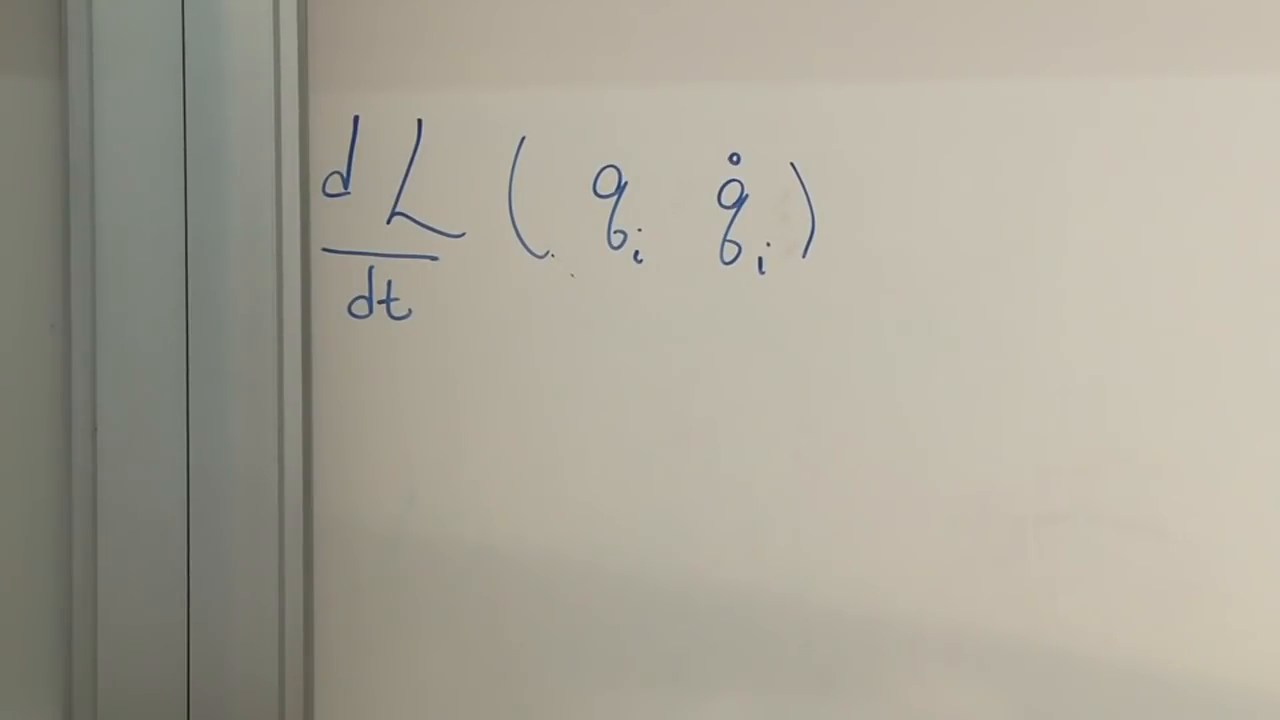
\includegraphics[width=0.72\textwidth]{lecture_05_figure_02.png}
  \caption{Начало вычисления производной \(L(q_i,\dot q_i)\) вдоль траектории.}
  \lectureframe{01:08:51}
\end{figure}

\begin{classroomqa}
  \audiencequestion{Не отсутствует ли в выражении по правилу цепочки знак суммирования?
  \lecturetimestamp{01:10:39--01:11:05}}
  \lecturerresponse{Да.  И каждая координата, и каждая скорость могут менять лагранжиан, поэтому оба члена суммируются по \(i\).}
\end{classroomqa}

Используем канонический импульс и уравнение Эйлера--Лагранжа,
\begin{equation}
  p_i=\frac{\partial L}{\partial\dot q_i},
  \qquad
  \dot p_i=\frac{\partial L}{\partial q_i}.
  \label{eq:l5-p-and-pdot}
\end{equation}
Тогда уравнение ~\eqref{eq:l5-chain-rule-no-time} принимает вид
\begin{align}
  \frac{dL}{dt}
  &=\sum_i(\dot p_i\dot q_i+p_i\ddot q_i)
  \notag\\
  &=\frac{d}{dt}\sum_i p_i\dot q_i.
  \label{eq:l5-product-rule}
\end{align}
Вся ``магия'' — это всего лишь правило произведения.

\begin{figure}[htbp]
  \centering
  \includegraphics[width=0.84\textwidth]{lecture_05_figure_21.png}
  \caption{Правило цепочки, преобразованное с помощью уравнений движения в производную от \(\sum_i p_i\dot q_i\).}
  \lectureframe{01:13:45}
\end{figure}

\begin{classroomqa}
  \audiencequestion{Должен ли последний \(q_i\) в произведении нести одну точку или две?
  \lecturetimestamp{01:14:31--01:15:32}}
  \lecturerresponse{Внутри произведения стоит \(p_i\dot q_i\), с одной точкой.  Дифференцирование произведения дает
  \(\dot p_i\dot q_i+p_i\ddot q_i\), что и объясняет две точки в развернутом втором члене.}
\end{classroomqa}

Вычитая эти две производные, получаем сохраняющуюся комбинацию. По исторической традиции берут величину с противоположным знаком и называют её гамильтонианом:
\begin{equation}
  H=\sum_i p_i\dot q_i-L.
  \label{eq:l5-hamiltonian-definition}
\end{equation}

\begin{figure}[htbp]
  \centering
  \includegraphics[width=0.80\textwidth]{lecture_05_figure_22.png}
  \caption{Сохраняющаяся комбинация \(L-\sum_i p_i\dot q_i=-H\) и определение гамильтониана.}
  \lectureframe{01:18:05}
\end{figure}

Для одной частицы в потенциале,
\begin{equation}
  L=\frac12m\dot x^2-V(x),
  \qquad p=m\dot x.
  \label{eq:l5-particle-lagrangian}
\end{equation}
Следовательно,
\begin{align}
  H&=p\dot x-L
  \notag\\
   &=m\dot x^2-\left(\frac12m\dot x^2-V(x)\right)
  \notag\\
   &=\frac12m\dot x^2+V(x)=T+V.
  \label{eq:l5-particle-energy}
\end{align}

\begin{figure}[htbp]
  \centering
  \includegraphics[width=0.86\textwidth]{lecture_05_figure_23.png}
  \caption{Гамильтониан частицы в потенциале сводится к привычной сумме кинетической и потенциальной энергий.}
  \lectureframe{01:20:50}
\end{figure}

При выводе не предполагалась никакая конкретная форма \(L\). Поэтому уравнение~\eqref{eq:l5-hamiltonian-definition}, а не \(T+V\), является общим определением энергии в этом формализме.

\section{Явная зависимость от времени и обмен энергией}

Восстановим явную зависимость от времени в правиле цепочки:
\begin{equation}
  \frac{dL}{dt}
  =\sum_i\left(
    \frac{\partial L}{\partial q_i}\dot q_i
    +\frac{\partial L}{\partial\dot q_i}\ddot q_i
  \right)
  +\frac{\partial L}{\partial t}.
  \label{eq:l5-full-chain-rule}
\end{equation}
Левая часть есть полная производная вдоль движения. Последняя частная производная берётся при фиксированных \(q\) и \(\dot q\) и дифференцирует только внешне изменяющиеся параметры. Повторяя тот же шаг с правилом произведения, получаем
\begin{equation}
  \boxed{\frac{dH}{dt}=-\frac{\partial L}{\partial t}}.
  \label{eq:l5-hamiltonian-time}
\end{equation}

\begin{figure}[htbp]
  \centering
  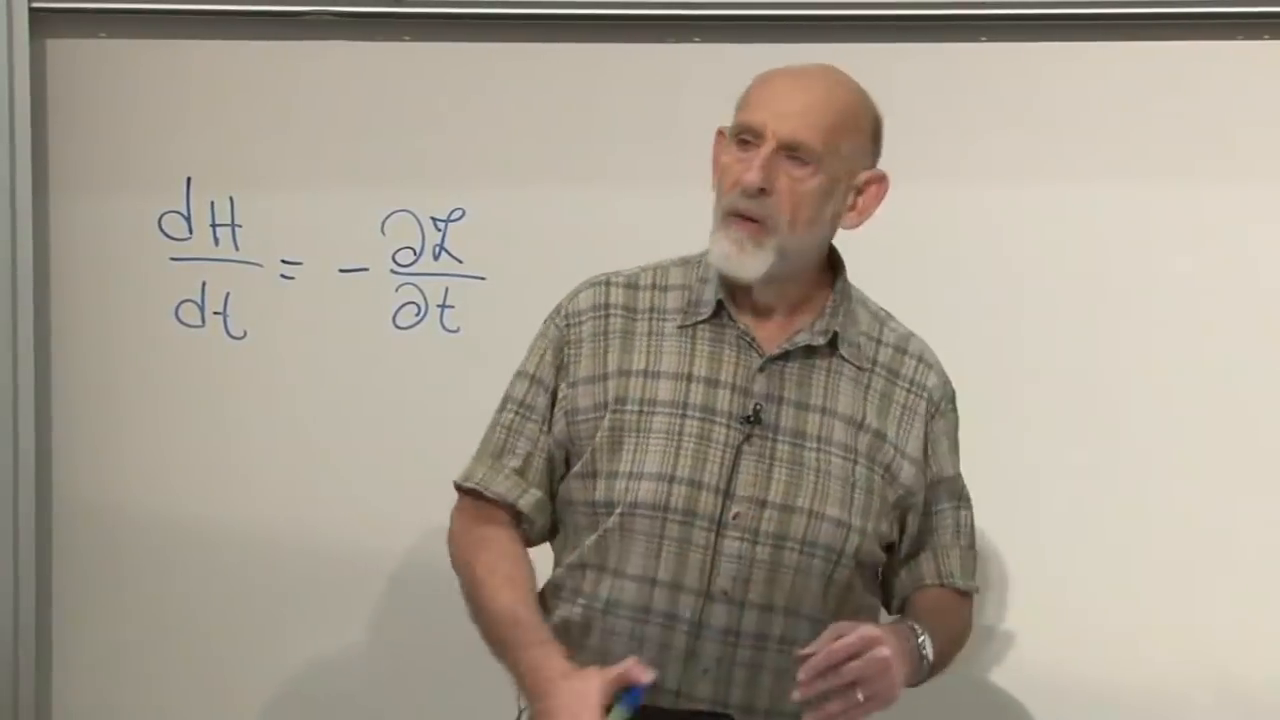
\includegraphics[width=0.70\textwidth]{lecture_05_figure_04.png}
  \caption{Гамильтониан изменяется только из-за явной зависимости лагранжиана от времени.}
  \lectureframe{01:37:22}
\end{figure}

Для вынужденного осциллятора из уравнения~\eqref{eq:l5-driven-oscillator},
\begin{equation}
  \frac{\partial L}{\partial t}
  =-\frac12\dot k(t)x^2,
  \qquad
  \dot H=\frac12\dot k(t)x^2.
  \label{eq:l5-driven-energy-rate}
\end{equation}
При \(x=0\) мгновенная производная обращается в нуль; вне начала координат изменение жёсткости пружины совершает работу с мощностью, пропорциональной \(x^2\dot k\).

\begin{classroomqa}
  \audiencequestion{Если энергия не сохраняется, не является ли её определением производная гамильтониана по времени?
  \lecturetimestamp{01:27:11--01:28:04}}
  \lecturerresponse{Нет. Энергия — это \(H\). Производная этой величины показывает, как она меняется. Когда лагранжиан имеет привычный вид, \(H=T+V\); когда нет, определение задаётся уравнением~\eqref{eq:l5-hamiltonian-definition}. Если расширить систему, включив внешний источник, восстановится сохранение полного гамильтониана.}
\end{classroomqa}

\begin{classroomqa}
  \audiencequestion{Как это применить к рассмотренному ранее наблюдателю на вращающейся карусели, где появились центробежные и кориолисовы члены?
  \lecturetimestamp{01:28:08--01:29:52}}
  \lecturerresponse{Равномерно вращающаяся система координат — это зависящая от времени замена переменных, а не фиксированная пространственная симметрия и не простой сдвиг по времени. Её преобразованный лагранжиан можно использовать для построения гамильтониана, но этот отдельный расчёт лучше отложить до обсуждения магнитных сил, поскольку соответствующая алгебра имеет очень близкую форму.}
\end{classroomqa}

\section{Лагранжев инструментарий в одном месте}

Теперь всю структуру можно записать в виде компактного набора:
\begin{align}
  L&=L(q_i,\dot q_i,t),
  \notag\\
  p_i&=\frac{\partial L}{\partial\dot q_i},
  \qquad
  \dot p_i=\frac{\partial L}{\partial q_i},
  \notag\\
  \delta q_i&=\epsilon f_i(q)
  \quad\Longrightarrow\quad
  Q=\sum_i p_i f_i(q),\quad \dot Q=0,
  \notag\\
  H&=\sum_i p_i\dot q_i-L,
  \qquad
  \dot H=-\frac{\partial L}{\partial t}.
  \label{eq:l5-toolkit}
\end{align}

\begin{figure}[htbp]
  \centering
  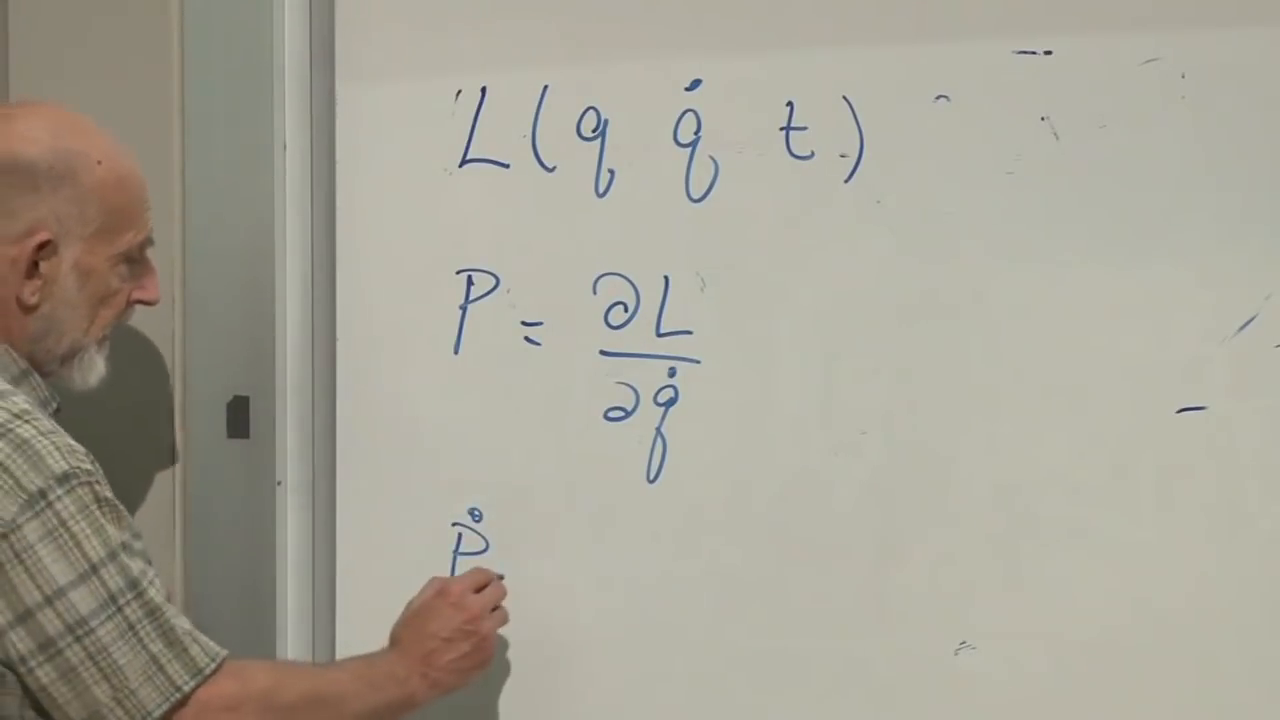
\includegraphics[width=0.66\textwidth]{lecture_05_figure_03.png}
  \caption{Краткое резюме на доске начинается с \(L(q,\dot q,t)\), канонического импульса и уравнения Эйлера--Лагранжа.}
  \lectureframe{01:31:37}
\end{figure}

Эти формулы содержат определение, уравнения движения, заряд обычной непрерывной симметрии и заряд трансляции по времени. Здесь почти нет хитростей; важно уметь заново выводить их, а не заучивать разрозненные выражения.

\section{Зачем использовать лагранжеву или гамильтонову механику?}

\begin{classroomqa}
  \audiencequestion{Можно ли в равной мере описывать механику с помощью \(L\) или \(H\), и почему выбирать ту или иную формулировку?
  \lecturetimestamp{01:37:16--01:39:18}}
  \lecturerresponse{Они эквивалентны, когда преобразование Лежандра регулярно, но подчёркивают разные структуры. Лагранжева механика естественно начинается с принципа стационарного действия. Гамильтонова механика поначалу более абстрактна, но её уравнения просты, и в квантовой механике она становится центральной. Гамильтониан — это энергия, но его роль гораздо шире, чем один только закон сохранения.}
\end{classroomqa}

\begin{classroomqa}
  \audiencequestion{Знал ли Ньютон гамильтонову форму закона сохранения энергии?
  \lecturetimestamp{01:39:29--01:39:56}}
  \lecturerresponse{Судя по историческим свидетельствам, не в этой формулировке. Ньютон формулировал механику на основе закона силы \(F=ma\).}
\end{classroomqa}

\begin{classroomqa}
  \audiencequestion{Почему всякая физическая система должна обладать лагранжианом? Это просто экспериментальный факт?
  \lecturetimestamp{01:39:57--01:42:37}}
  \lecturerresponse{Для рассматриваемых замкнутых систем это эмпирический факт и, кроме того, следствие более глубокого квантового описания. Можно придумать математически непротиворечивые дифференциальные уравнения, которые не являются уравнениями Эйлера--Лагранжа. Например, \(\dot x=-x\) прекрасно решается, но как фундаментальный закон для замкнутой системы с одной координатой оно имеет диссипативный характер с потерей информации. Классическая механика не предшествует квантовой механике логически; её фундаментальная структура унаследована от квантовой механики. Подробное объяснение придётся отложить.}
\end{classroomqa}

\begin{classroomqa}
  \audiencequestion{Если у всякой реальной замкнутой системы есть лагранжиан, то соответствует ли каждая функция, которую мы называем лагранжианом, системе, встречающейся в природе?
  \lecturetimestamp{01:42:39--01:42:54}}
  \lecturerresponse{Нет. Формальное исчисление допускает много функций, которые не реализуются ни в одной известной физической системе.}
\end{classroomqa}

\begin{classroomqa}
  \audiencequestion{Является ли лагранжиан главным образом инструментом для придумывания потенциалов?
  \lecturetimestamp{01:42:54--01:43:32}}
  \lecturerresponse{Его роль шире. Он может служить для систематизации возможных механических систем и часто является кратчайшим практическим путём к уравнениям движения.}
\end{classroomqa}

Двойной маятник демонстрирует это практическое преимущество. Выберите два угла, вычислите скорости обеих масс через эти углы и их производные по времени, составьте \(T-V\), и пусть уравнения Эйлера--Лагранжа неявно учтут силы связи. Это значительно чище, чем разбирать все натяжения и ускорения с помощью \(F=ma\).

\begin{figure}[htbp]
  \centering
  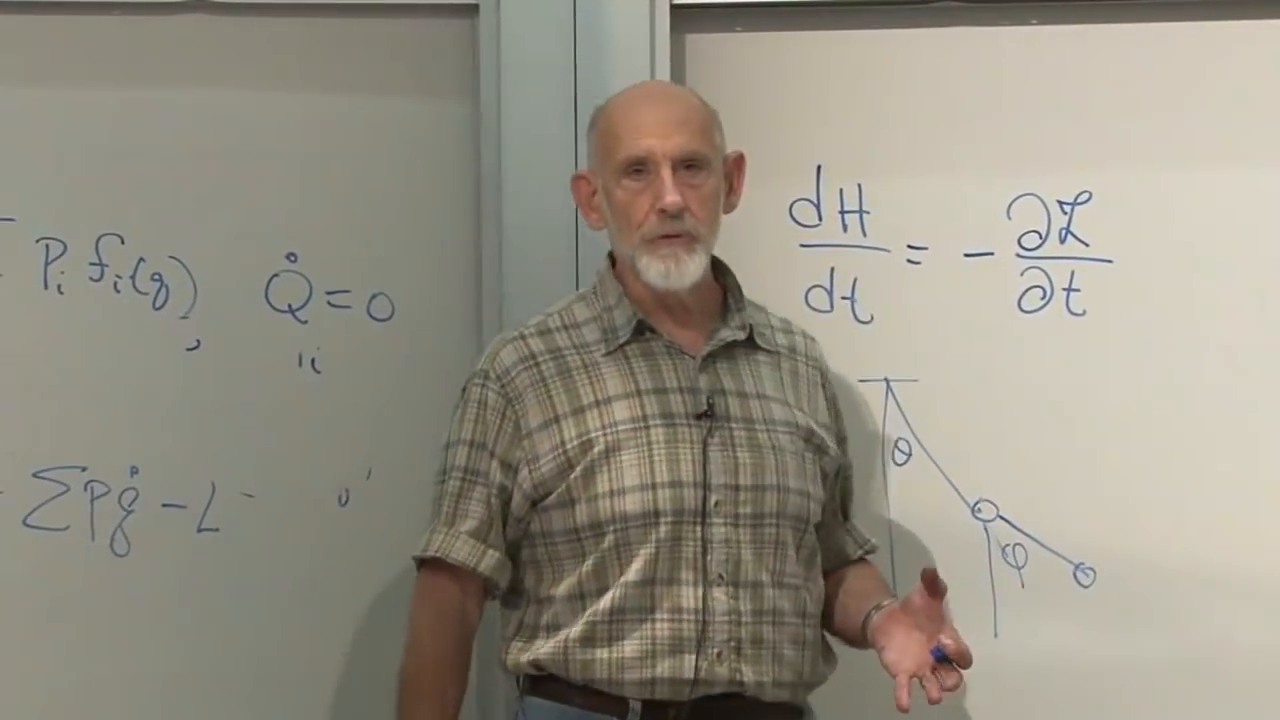
\includegraphics[width=0.84\textwidth]{lecture_05_figure_05.png}
  \caption{Соотношение для скорости изменения энергии остаётся на доске рядом с рисунком двойного маятника.}
  \lectureframe{01:45:39}
\end{figure}

\begin{figure}[htbp]
  \centering
  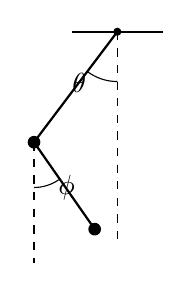
\begin{tikzpicture}[scale=1.15]
    \draw[thick] (-0.5,0) -- (0.5,0);
    \fill (0,0) circle (0.045);
    \draw[dashed] (0,0) -- (0,-2.3);
    \draw[thick] (0,0) -- (-0.92,-1.22);
    \fill (-0.92,-1.22) circle (0.07);
    \draw[dashed] (-0.92,-1.22) -- (-0.92,-2.55);
    \draw[thick] (-0.92,-1.22) -- (-0.25,-2.18);
    \fill (-0.25,-2.18) circle (0.07);
    \draw (0,-0.55) arc (-90:-127:0.55);
    \node at (-0.42,-0.56) {$\theta$};
    \draw (-0.92,-1.72) arc (-90:-55:0.48);
    \node at (-0.56,-1.72) {$\phi$};
  \end{tikzpicture}
  \caption{Обобщённые угловые координаты двойного маятника.}
\end{figure}

Замена переменных столь же эффективна: преобразуйте один лагранжиан, а затем выведите его уравнения, вместо того чтобы по отдельности преобразовывать каждое уравнение в терминах сил.

\begin{classroomqa}
  \audiencequestion{Является ли двойной маятник по существу ещё одной системой трёх тел, такой как Солнце, Земля и Луна, где одно тело рассматривается как опора?
  \lecturetimestamp{01:45:06--01:45:25}}
  \lecturerresponse{Эта аналогия передаёт иерархию, хотя стержни накладывают другие связи. В обоих случаях очень массивную или закреплённую составляющую можно в приближении рассматривать как опорную структуру.}
\end{classroomqa}

\begin{classroomqa}
  \audiencequestion{В двойном маятнике используется \(T-V\), хотя только что подчёркивалась важность более общих лагранжианов. Когда справедливо \(T-V\)?
  \lecturetimestamp{01:46:08--01:46:58}}
  \lecturerresponse{Для обычных нерелятивистских частиц в инерциальной системе отсчёта, при отсутствии магнитной связи, зависящей от скорости, применима привычная форма. Вращающиеся системы отсчёта, релятивистские системы и магнитные поля требуют более общих членов.}
\end{classroomqa}

\begin{classroomqa}
  \audiencequestion{Выходят ли столкновения за пределы этого описания?
  \lecturetimestamp{01:47:00--01:48:05}}
  \lecturerresponse{Упругие столкновения возникают из-за короткодействующих сил и, следовательно, из потенциалов. Неупругие столкновения на микроскопическом уровне всё равно остаются механическими, но энергия уходит во внутренние колебания, деформацию и тепло. Описание через центр масс, опускающее эти степени свободы, неполно.}
\end{classroomqa}

\begin{classroomqa}
  \audiencequestion{Можно ли анализировать бейсбольный мяч, по которому ударили битой, с помощью \(F=ma\)?
  \lecturetimestamp{01:48:05--01:48:33}}
  \lecturerresponse{Лишь на грубом уровне. Полное описание должно отслеживать деформацию, нагрев, возможное повреждение мяча и, возможно, поломку биты. Именно из-за этих внутренних степеней свободы реалистичный удар намного сложнее, чем столкновение точечных частиц.}
\end{classroomqa}

\begin{classroomqa}
  \audiencequestion{А как насчёт протяжённого твёрдого тела?
  \lecturetimestamp{01:48:34--01:49:00}}
  \lecturerresponse{Твёрдые тела можно изучать либо ньютоновскими методами, либо с помощью лагранжиана \(T-V\), записанного в поступательных и вращательных координатах. Построение такого лагранжиана — полезное упражнение.}
\end{classroomqa}

\begin{classroomqa}
  \audiencequestion{Означает ли квантовое соотношение неопределённостей энергия--время, что энергия не сохраняется строго?
  \lecturetimestamp{01:49:01--01:49:29}}
  \lecturerresponse{Нет. Энергия может сохраняться строго. Это соотношение говорит, что для определения энергии с высокой точностью требуется наблюдение в течение длительного времени; оно не заменяет закон сохранения.}
\end{classroomqa}

\begin{classroomqa}
  \audiencequestion{Ньютонова и лагранжева механика логически эквивалентны?
  \lecturetimestamp{01:49:36--01:50:07}}
  \lecturerresponse{Они эквивалентны в обычной области, где применимы обе формулировки. Тем не менее можно построить лагранжианы, чьи уравнения не похожи на элементарную форму \(m\ddot x=F(x)\).}
\end{classroomqa}

\section{Кинетический член с координатной зависимостью}

Рассмотрим намеренно непривычный пример
\begin{equation}
  L=\frac12q^2\dot q^2-\frac12q^2.
  \label{eq:l5-nonstandard-l}
\end{equation}
Это корректный лагранжиан с зависящим от координаты коэффициентом при кинетическом члене. Можно было бы рассмотреть и члены, линейные по скорости, такие как \(q\dot q\); в этом одномерном примере данный член является полной производной и не изменил бы уравнения движения.

Канонический импульс равен
\begin{equation}
  p=\frac{\partial L}{\partial\dot q}=q^2\dot q,
  \label{eq:l5-nonstandard-p}
\end{equation}
так что
\begin{equation}
  \dot p=q^2\ddot q+2q\dot q^2,
  \qquad
  \frac{\partial L}{\partial q}=q\dot q^2-q.
  \label{eq:l5-nonstandard-derivatives}
\end{equation}
Поэтому уравнение движения имеет вид
\begin{equation}
  q^2\ddot q+q\dot q^2=-q.
  \label{eq:l5-nonstandard-eom}
\end{equation}

\begin{figure}[htbp]
  \centering
  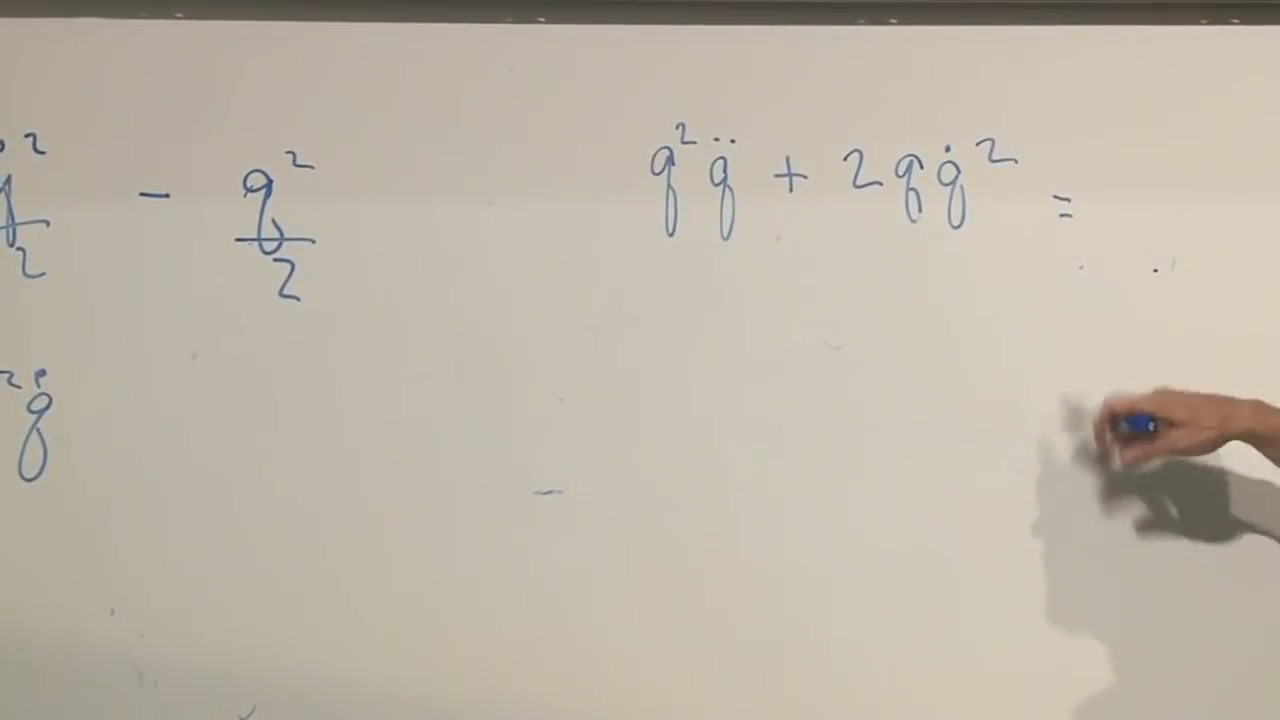
\includegraphics[width=0.80\textwidth]{lecture_05_figure_06.png}
  \caption{Производная импульса в примере с зависящим от координаты коэффициентом при кинетическом члене.}
  \lectureframe{01:52:32}
\end{figure}

\begin{classroomqa}
  \audiencequestion{Можно ли разделить уравнение на \(q\)?
  \lecturetimestamp{01:53:22--01:53:39}}
  \lecturerresponse{Только там, где \(q\neq0\). При \(q=0\) кинетический коэффициент и отображение Лежандра вырождены, поэтому деление отбросило бы особую точку, требующую отдельного рассмотрения.}
\end{classroomqa}

Гамильтониан равен
\begin{align}
  H&=p\dot q-L
  \notag\\
   &=q^2\dot q^2-
     \left(\frac12q^2\dot q^2-\frac12q^2\right)
  \notag\\
   &=\frac12q^2\dot q^2+\frac12q^2.
  \label{eq:l5-nonstandard-h}
\end{align}

\begin{classroomqa}
  \audiencequestion{Можно ли по-прежнему называть \(q^2\dot q^2/2\) кинетической энергией?
  \lecturetimestamp{01:54:41--01:55:07}}
  \lecturerresponse{Да. В этом разобранном примере гамильтониан снова выглядит как сумма положительного кинетического члена и потенциального члена. Суть в том, что формальные определения сработали без предварительного предположения о простейшей форме с постоянной массой.}
\end{classroomqa}

\section{Диссипация и более глубокое происхождение формализма}

\begin{classroomqa}
  \audiencequestion{Как включить трение в лагранжиан?
  \lecturetimestamp{01:55:09--01:56:17}}
  \lecturerresponse{Не в качестве фундаментальной силы в рассматриваемой здесь простой замкнутой системе с конечным числом степеней свободы. Макроскопическое трение представляет собой статистический эффект огромного числа микроскопических степеней свободы. Эти атомы по-прежнему подчиняются лежащей в основе механике, но в редуцированном описании, которое их не отслеживает, проявляется диссипация.}
\end{classroomqa}

\begin{classroomqa}
  \audiencequestion{Как Hamilton пришёл к своей формулировке?
  \lecturetimestamp{01:56:22--01:56:37}}
  \lecturerresponse{Здесь не приводилось исторического вывода. Важная задача для данного курса — понять, как работает эта формулировка.}
\end{classroomqa}

\begin{classroomqa}
  \audiencequestion{Есть ли более общий рецепт получения лагранжиана, когда он не имеет очевидного вида \(T-V\)?
  \lecturetimestamp{01:56:43--01:58:54}}
  \lecturerresponse{Эту функцию могут дать эксперимент, обоснованная догадка, принцип симметрии или восстановление из желаемых уравнений. Спрашивать у самого исчисления, откуда берётся его вход, — всё равно что спрашивать у определения производной, откуда взялась \(f(x)\). Исчисление говорит, что делать, когда функция уже задана. На более глубоком уровне на вопрос о том, почему замкнутые системы природы подчиняются этой абстрактной структуре, отвечает квантовая механика.}
\end{classroomqa}

Этот момент связан с темами, затронутыми в начале курса. Фундаментальная гамильтонова эволюция детерминистична и обратима в том смысле, что траектории не сливаются и информация не просто уничтожается. Связь между этим свойством и формулировкой в фазовом пространстве будет раскрываться постепенно.

\begin{classroomqa}
  \audiencequestion{Не сводилось ли вариационное исчисление просто к обратному ходу от желаемых классических уравнений, и получает ли квантовая механика свой лагранжиан тем же путём?
  \lecturetimestamp{01:59:37--02:01:07}}
  \lecturerresponse{В элементарном классическом построении действительно можно выбрать действие, стационарные траектории которого воспроизводят известные уравнения. Логический порядок в квантовой механике иной: она естественным образом начинается с гамильтониана и может переходить к лагранжеву описанию. Гамильтониан там более интуитивен, хотя в классической механике поначалу кажется абстрактным.}
\end{classroomqa}

\begin{classroomqa}
  \audiencequestion{Может ли квантовая механика описывать трение?
  \lecturetimestamp{02:01:08--02:02:05}}
  \lecturerresponse{Да, но фундаментальное описание должно включать степени свободы окружения. Частицу, движущуюся в вязкой жидкости, невозможно полностью описать без частиц самой жидкости. Трение — это сложный коллективный эффект, возникающий, когда за этими степенями свободы не следят по отдельности.}
\end{classroomqa}